\begin{figure}[htbp]
    \centering
    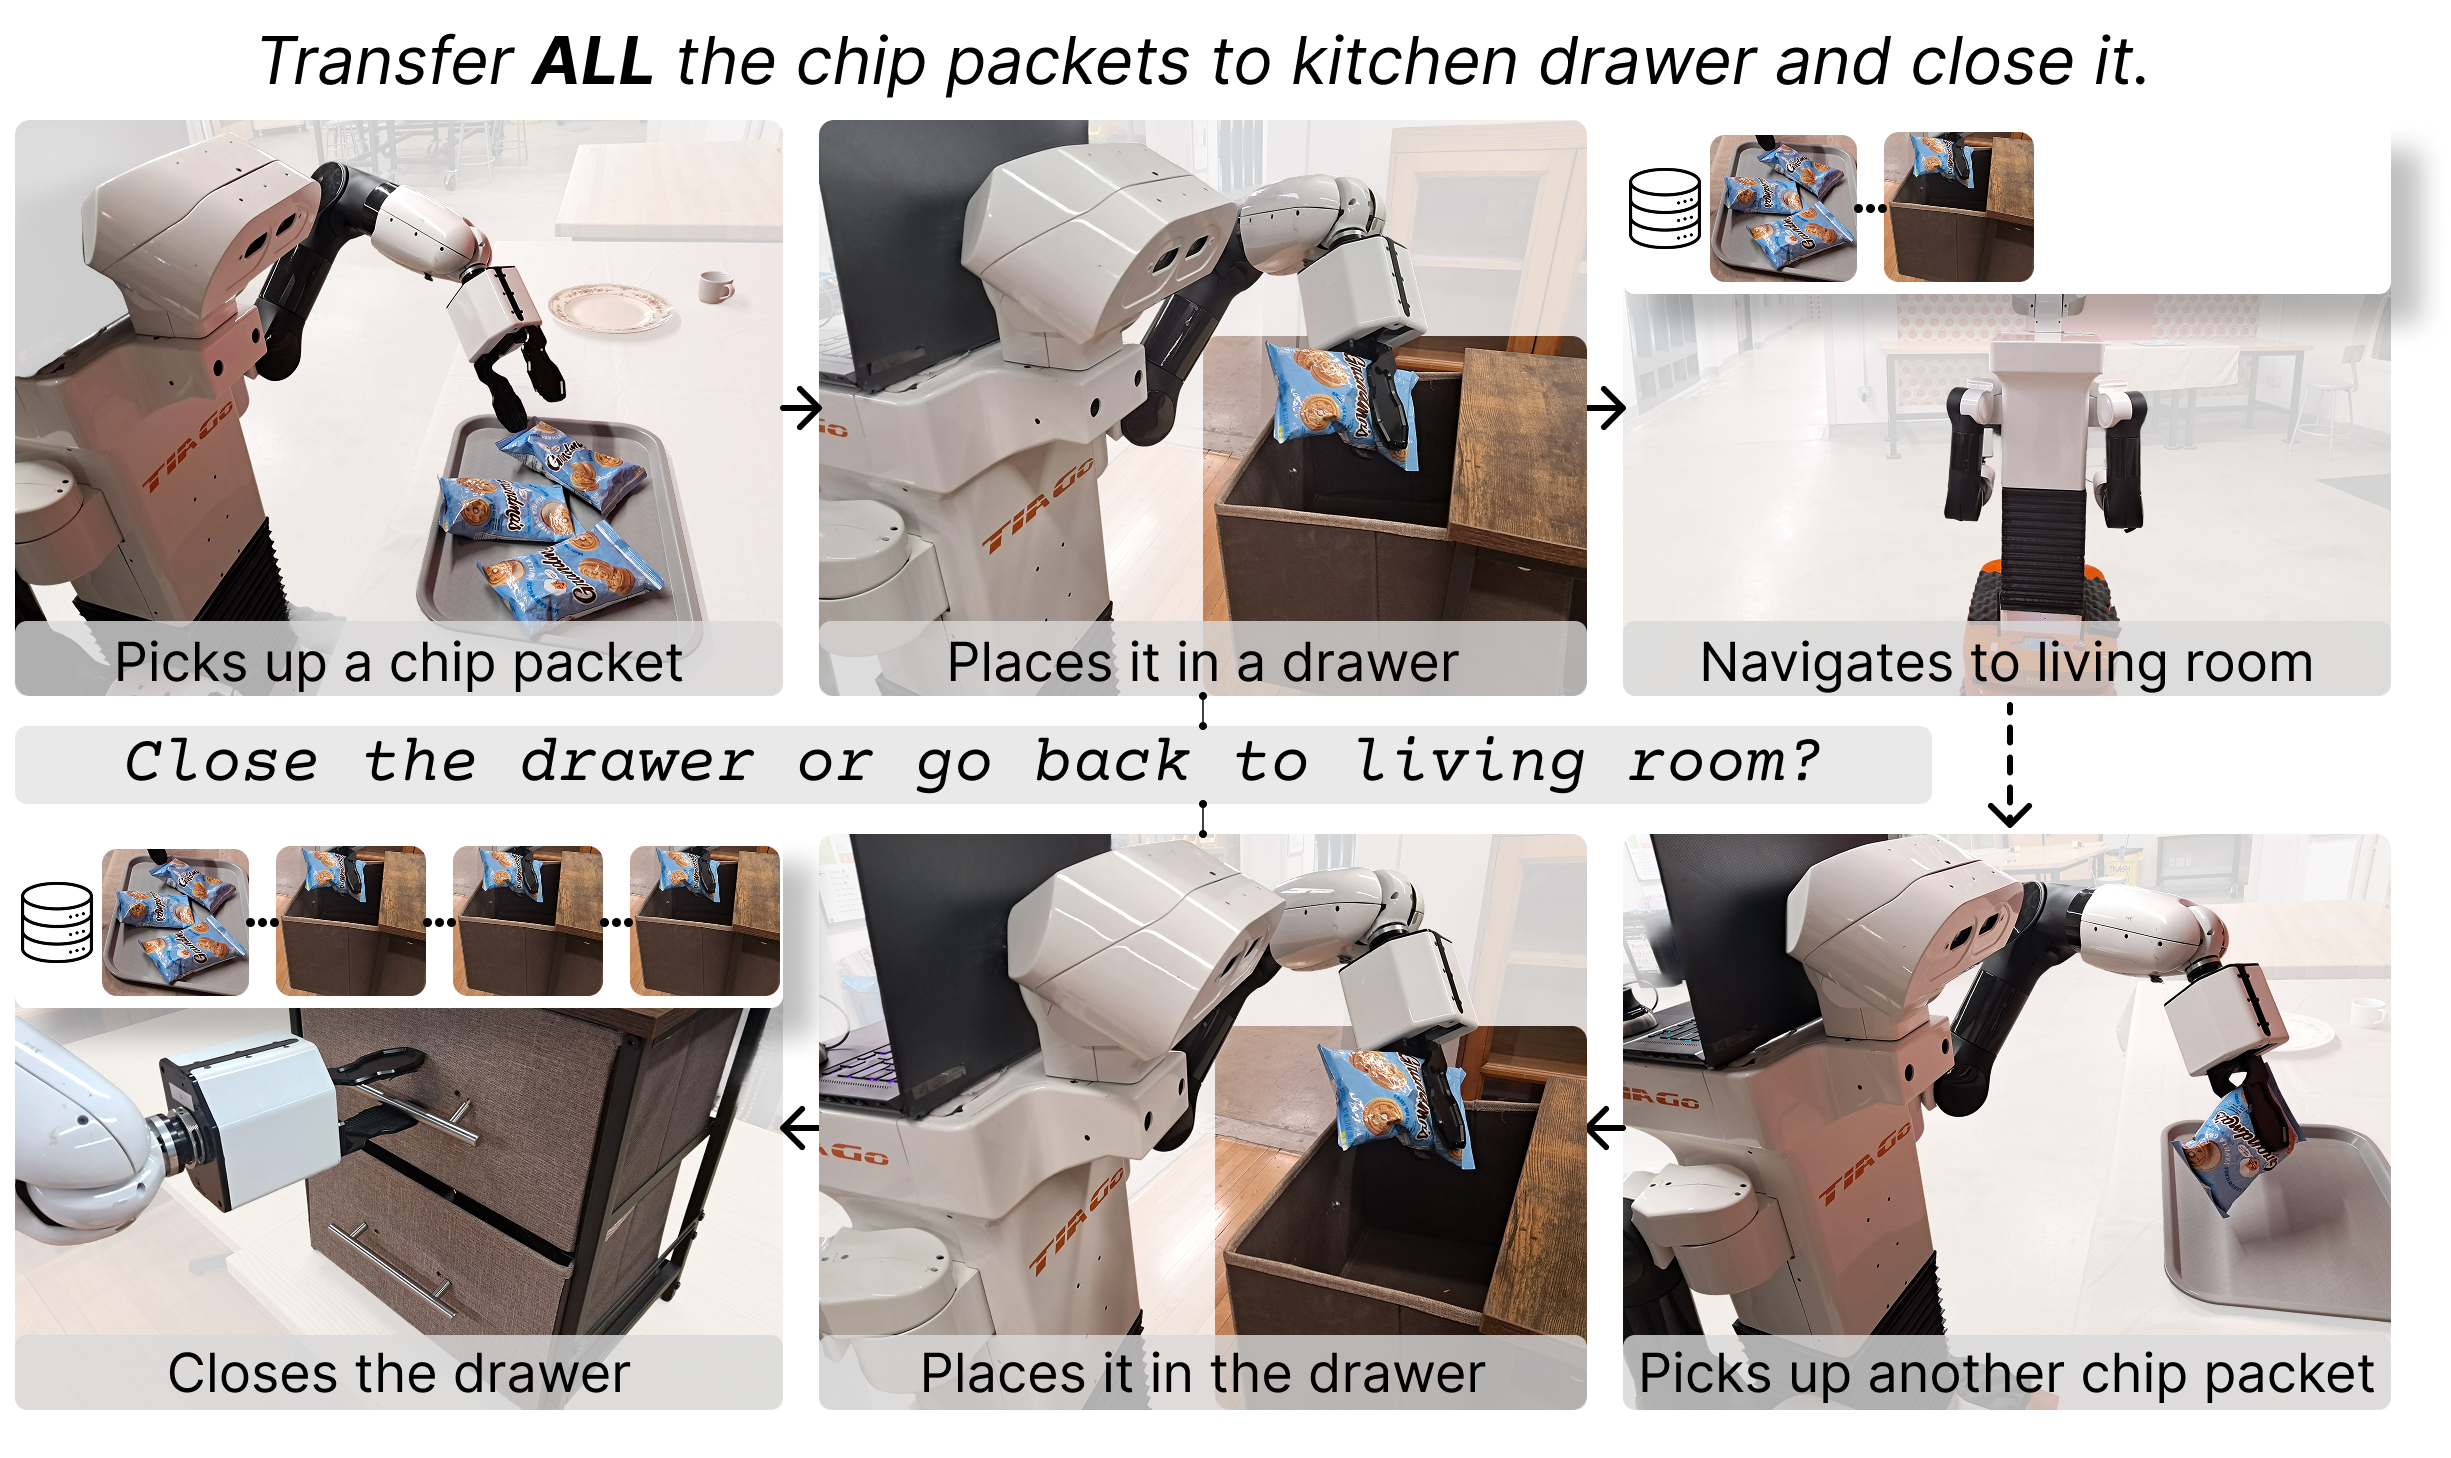
\includegraphics[width=0.5\textwidth, trim=0 0.5cm 0 0, clip]{figures/pull_figurev3.png}
    \vspace{-20pt}
    \caption{\textbf{Memory retrieval in visuomotor policy learning.} Long-horizon household tasks require robots to act on information no longer present in the current sensory input. Under partial observability, the policy must retrieve relevant information from past observations stored in memory to predict correct low-level actions. The type of information needed can change across task stages, motivating a general, learned retrieval mechanism.}
    \label{fig:pull_figure}
    \vspace{-10pt}
\end{figure}
